\documentclass[tikz,margin=1cm]{standalone}

\usepackage{pgfplots}
\pgfplotsset{compat=1.16}
\usepgfplotslibrary{fillbetween}


\begin{document}
        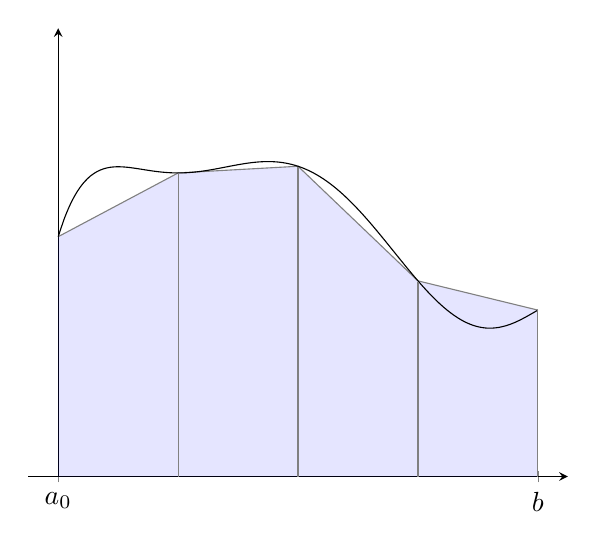
\begin{tikzpicture}
            \begin{axis}[
                axis equal,
                grid=none,
                domain=0:8,
                samples=75,
                ymin=0,
                xmax=8.5,
                xmin=-0.5,
                axis lines = middle,
                axis x line = bottom,
                xtick={0,8},
                ytick={0},
                xticklabels={$a_0$,$b$},
                % xlabel=$x$,
                % ylabe$$l=$y$,
                ]
                    \path[name path=axis] (axis cs:0,0) -- (axis cs:8,0);

                \addplot[samples=5, gray, name path=tr] {(-0.00128205128205*x^6+0.0341538461538*x^5-0.337980769231*x^4+1.54115384615*x^3-3.365*x^2+3.29538461538*x)+4};
                \addplot[smooth] {(-0.00128205128205*x^6+0.0341538461538*x^5-0.337980769231*x^4+1.54115384615*x^3-3.365*x^2+3.29538461538*x)+4};
                    \addplot [
        thick,
        color=blue,
        fill=blue, 
        fill opacity=0.10
    ]
    fill between[
        of=tr and axis,
        soft clip={domain=0:8},
    ];

                \addplot[gray] coordinates {(2, 0) (2, 5.05)};
                \addplot[gray] coordinates {(4, 0) (4, 5.17)};
                \addplot[gray] coordinates {(6, 0) (6, 3.25)};
                \addplot[gray] coordinates {(8, 0) (8, 2.77)};
            \end{axis}
        \end{tikzpicture}
\end{document}
